\tableofcontents

\printnoidxglossary[type=\acronymtype,title=List of Abbreviations]
\listoffigures

\mainmatter

\hypertarget{introduction}{%
\chapter{Introduction}\label{introduction}}

\hypertarget{related-work}{%
\chapter{Related work}\label{related-work}}

In this chapter we will provide a high level overview of relevant
solutions for connecting the parties of an MPyC multiparty computation
over the internet. We will use the \gls{osi} model to help us categorize
those solutions and highlight the similarities and differences between
them. The OSI model has 7 layers with different responsibilities:

\begin{description}
\item[Layer 7 - Application:]
high level protocols that interact with user-facing services
\item[Layer 6 - Presentation:]
translation of data between a networking service and an application,
e.g.~encoding, compression, encryption
\item[Layer 5 - Session:]
session setup, management, tear-down, authentication, authorization
\item[Layer 4 - Transport:]
sending data of variable length over a network while maintaining
quality-of-service, e.g.~ports, connections, packet fragmentation
\item[Layer 3 - Network:]
sending data packets between two nodes, routed via a path of other
nodes, e.g.~addressing, routing
\item[Layer 2 - Data link:]
sending data frames between two nodes, directly connected via a physical
layer, e.g.~on a LAN
\item[Layer 1 - Physical:]
sending raw bits over a physical medium
\end{description}

While many protocols implement aspects of several layers and do not
strictly fit inside the OSI model, it still a useful visualization tool.
The diagram below shows an approximate OSI model mapping of several
protocols and network overlay solutions from the point of view of the
systems that use them and the arrows show dependency relations between
them.

\newpage

\begin{figure}
\centering
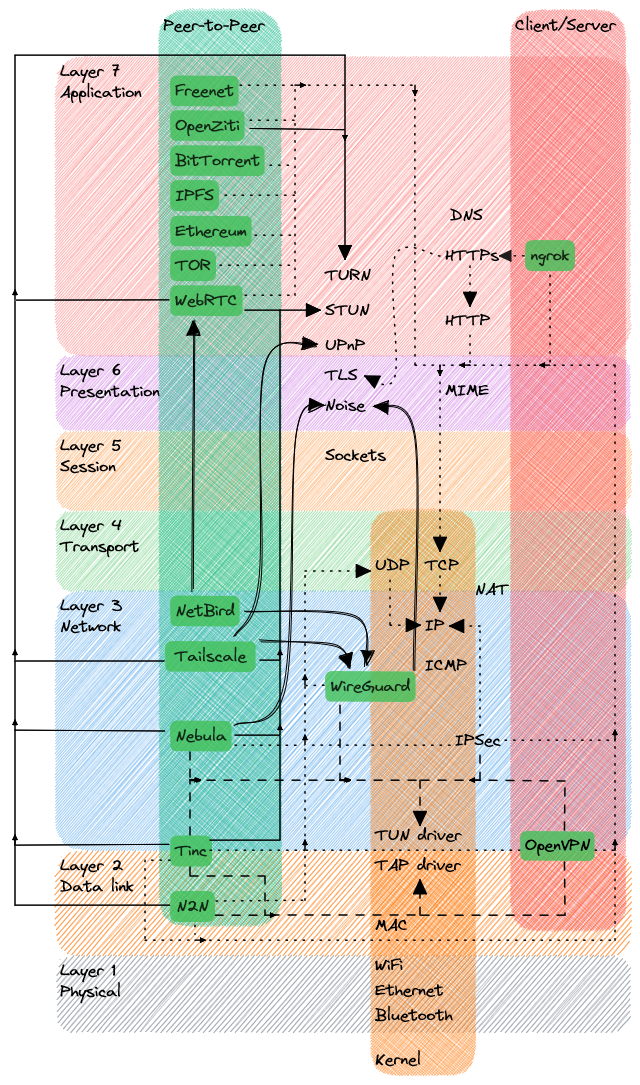
\includegraphics[width=\textwidth,height=0.9\textheight]{thesis/../Excalidraw/osi-map.excalidraw.png}
\caption{OSI model mapping of various protocols \label{osiMap}}
\end{figure}

\hypertarget{the-internet}{%
\section{The Internet}\label{the-internet}}

The modern Internet is a global multi-tiered network of devices that
communicate using the protocols of the Internet Protocol Suite (TCP/IP).
Typically, an \gls{isp} manages the physical infrastructure that
connects an end-user's devices with the rest of the internet.

The \textbf{\acrfull{ip}} is a Network (Layer 3) protocol of the
Internet Protocol Suite that is responsible for delivering datagrams
between devices across the boundaries of their \glspl{lan} by possibly
routing traffic via multiple intermediate devices (routers). A datagram
is a connectionless packet that is delivered on a best effort basis. It
has a header that contains fields such as the \textbf{IP addresses} of
its source and destination, and a payload that encapsulates the data
from the protocols of the layers above. Routers are devices that are
part of multiple networks and relay datagrams between them based on a
routing table that maps IP address ranges (\gls{cidr}) to networks.

\textbf{\acrfull{udp}} and \textbf{\acrfull{tcp}} are Transport (Layer
4) protocols that add the concept of ports to allow having multiple
communication channels simultaneously between two devices. UDP provides
best-effort delivery, while TCP is a reliable transport with delivery
guarantees. TCP maintains stateful connections and handles
acknowledgements and retransmissions in case of packets lost in transit.

\textbf{\acrfull{tls}} is a protocol that adds encryption on top of a
reliable transport protocol such as TCP. It is usually placed in the
Presentation Layer (Layer 6), but it does not strictly fit in any single
OSI layer. It is rather complex because it needs to support many
possible use cases across the internet. \todo{tls} The \textbf{Noise
Protocol Framework} \autocite{noiseDocs} is a more
\todo{noise is transport agnostic}
\todo{noise has limited cipher suites} recent effort that applies the
ideas of TLS in a simplified way by serving as a blueprint for designing
use-case specific protocols for establishing secure communication
channels based on \gls{ecdh} handshake patterns. It powers the
end-to-end encryption in messaging applications such as WhatsApp and
Signal, and \gls{vpn} software such as WireGuard and Nebula.

The version of the Internet Protocol that was originally deployed
globally (IPv4) uses 32-bit numbers as IP addresses, allowing for up to
4, 294, 967, 296 unique addresses. Due to the popularity of the
internet, there are many more devices than available IPv4 addresses,
which has caused challenges. IPv6 is a newer version of the protocol
that uses a larger 128-bit address space, but it's adoption has been
slow. A more widespread solution is \textbf{\gls{nat}}. It allows many
devices without globally unique IP addresses to initiate connections to
publicly addressable devices on the Internet via a limited number of
gateways that must have globally unique IP addresses. A NAT gateway
replaces the local source IP address of each outgoing IP datagram with
its own public IP address before passing it on to the next link on the
way to the destination while maintaining a mapping between the source
and destination IPs in a translation table. The destination host can
then address its responses back to the NAT gateway's public IP address,
which in turn replaces its own IP from the incoming datagrams with the
IP of the local device and relays them to it. If the IP datagrams
encapsulate TCP/UDP packets, the gateway additionally rewrites the
source and destination ports, which means that NAT techniques can be
placed somewhere between Layers 3 and 4 of the OSI model.

The NAT approach allows devices with local IP addresses to initiate
bidirectional connections with remote devices across the public internet
but it does not natively allow those remote devices to initiate a
connection first. Furthermore as Figure \ref{nat-intro} shows, when two
different devices are behind separate NATs, neither can contact the
other one first, which causes problems for many Peer-to-Peer protocols.
There are several \textbf{NAT traversal} techniques that try to aleviate
this drawback with varying success and performance tradeoffs.

\begin{figure}
\centering
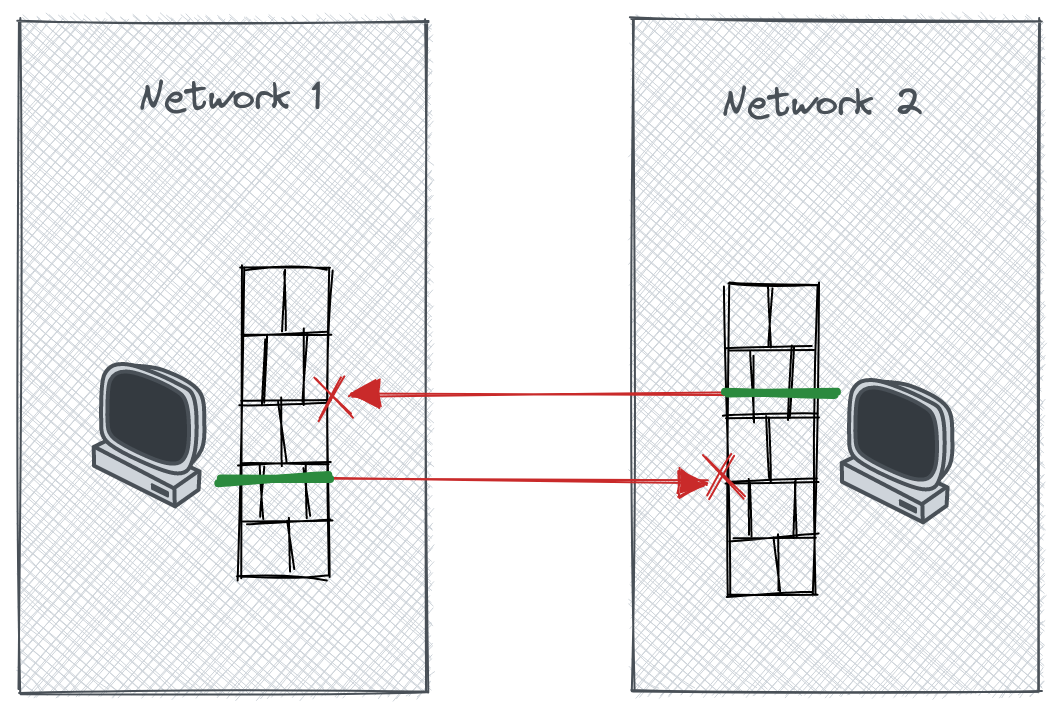
\includegraphics[width=0.5\textwidth,height=0.25\textheight]{thesis/../figures/nat-intro.png}
\caption{Two parties behind separate NATs\label{nat-intro}}
\end{figure}

In many home networks the role of a NAT gateway is played by a publicly
addressable router under the user's control, which often allows for port
forwarding to be configured either manually or programmatically via a
Layer 7 protocol like \textbf{\gls{upnp}} or its successors
\textbf{\gls{nat-pmp}} and \textbf{\gls{pcp}}. This would allow remote
hosts to initiate connections with the local ones if they know the
router's public IP address. Those protocols however are not always
supported by the router and are often disabled by the local network
administrators due to the security concerns of maliscious programs being
able to request and modify the port mappings in the router's translation
tables.

Another approach for NAT traversal is \textbf{\gls{stun}}, which relies
on the predictable port mapping algorithms that many routers use and a
public third party host that can be contacted by the local devices and
later serve as an introduction point for them (Figure
\ref{nat-traversal}).

\todo{rewrite this text from the preparation phase by separating the discussions of STUN and Mesh VPNs, which will be introduced in the next section after we've looked at the lower level protocols}

\begin{quote}
\gls{udp} hole punching based on concepts from \gls{stun}. The machines
of each party can contact a public \gls{stun} server
\ref{nat-traversal}, which will note what \gls{ip} addresses the
connections come from and inform the parties. Since the parties
initiated the connection to the STUN server, their routers will keep a
mapping between their local IP addresses and the port that was allocated
for the connection in order to be able to forward the incoming traffic.
Those ``holes'' in the NATs were originally intended for the STUN
server, but mesh VPNs use the stateless ``fire and forget'' UDP protocol
for their internal communication, which does not require nor provides a
mechanism for the NATs to verify who sent a UDP packet. With most NATs,
this is enough to be able to (ab)use the ``punched holes'' for the
purpose of \gls{p2p} traffic from other parties. Mesh VPNs implement the
stateful \gls{tcp} and \gls{tls} protocols on top of UDP and expose an
regular network interface to the other programs, keeping them shielded
from the underlying complexities. Other NAT implementations such as
Symmetric NAT and \glspl{cgnat} can be more difficult to ``punch
through'' due to their more complex port mapping strategies. In those
cases, establishing P2P connections might involve guess work or even
fail and require falling back to routing the (encrypted) traffic via
another party or service.
\end{quote}

\begin{figure}
\centering
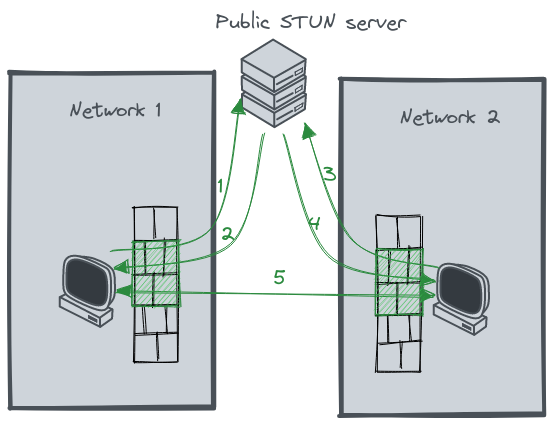
\includegraphics[width=0.5\textwidth,height=0.25\textheight]{thesis/../figures/nat-traversal.png}
\caption{NAT traversal via STUN\label{nat-traversal}}
\end{figure}

In most mobile networks (4G, 5G) the \gls{isp} utilizes a
\textbf{\gls{cgnat}} as part of their infrastructure, while all devices
under the user's control, including the router only have local IP
addresses. STUN techniques would fail to discover a direct path between
two parties behind separate CGNATs or other unpredictable NAT
algorithms. The only remaining possiblity is for a techniques like
\textbf{\acrfull{turn}}, where a publicly reachable third party host is
used not only for introducing the peers but also for relaying all
(possibly encrypted) traffic between them.

\begin{itemize}
\tightlist
\item
  \textbf{\acrfull{ipsec}}

  \begin{itemize}
  \tightlist
  \item
    Layer 3 protocol suite part of the Internet Protocol Suite
  \item
    used inside VPN software
  \item
    has implementations in both user and kernel space as well as
    hardware implementations
  \item
    rewrites and encrypts the IP headers and payloads
  \item
    virtual routing table
  \item
    Initially was built into IPv6, separate from IPv4
  \end{itemize}
\end{itemize}

\hypertarget{network-overlays}{%
\section{Network overlays}\label{network-overlays}}

Most Network Overlay solutions can be placed in Layers 2, 3 or 7.

\hypertarget{tuntap-driver}{%
\subsection{TUN/TAP driver}\label{tuntap-driver}}

\begin{itemize}
\tightlist
\item
  Layer 2 vs Layer 3 Networks

  \begin{itemize}
  \tightlist
  \item
    Layer 2 overlays bridge networks

    \begin{itemize}
    \tightlist
    \item
      virtual network switch
    \item
      remote machines are on the same virtual LAN and can share the same
      IP address range
    \item
      allows broadcast/multicast
    \item
      TAP driver
    \end{itemize}
  \item
    Layer 3 overlays route traffic between separate local networks

    \begin{itemize}
    \tightlist
    \item
      virtual network router
    \item
      remote machines are on separate LANs
    \item
      simpler to configure
    \item
      TUN driver
    \end{itemize}
  \end{itemize}
\end{itemize}

\hypertarget{traditional-vpns}{%
\subsection{Traditional VPNs}\label{traditional-vpns}}

\glspl{vpn} are implemented as Layer 2 or 3 network overlays. They are
commonly used for securely connecting machines from different
\glspl{lan}. They provide software emulation of a network interface
controller via a TUN/TAP driver on the operating system level and allow
other software to transparently use the functionality of the \gls{ip}
suite without requiring extra changes. Traditional \glspl{vpn} such as
IPSec \autocite{ipSecDocs} and OpenVPN \autocite{openVPNDocs} use a
centralized service that all (encrypted) client communications must pass
through. This introduces a single point of failure and a potential
bottleneck that might negatively impact the performance of the
multi-party computations due to their \gls{p2p} nature.

\hypertarget{wireguard}{%
\subsection{WireGuard}\label{wireguard}}

WireGuard \autocite{donenfeldWireGuardNextGeneration2017} is a more
recent protocol with a design informed by lessons learned from IPSec and
OpenVPN and a key management approach inspired by SSH. It is a lower
level protocol that focuses on configuration simplicity while network
topology, peer discovery and key distribution are left as a
responsibility of higher level systems that use it as a building block.
Wireguard is implemented as a Layer 3 overlay over UDP tunnels.
WireGuard has both user space implementations that use a TUN driver and
also has direct support built into the Linux Kernel since version 5.6
(May 2020). The kernel implementation allows for better performance
because it does not need to copy packets between the kernel and
user-space memory.

The snippets below show a minimal set of configuration options that need
to be provided in order for two peers to be able to form secure tunnels
with each other.

\begin{Shaded}
\begin{Highlighting}[]
\CommentTok{\# peer1.conf}
\KeywordTok{[Interface]}
\DataTypeTok{Address }\OtherTok{=}\StringTok{ 101.0.0.1/32}
\DataTypeTok{ListenPort }\OtherTok{=}\StringTok{ }\DecValTok{53063}
\DataTypeTok{PrivateKey }\OtherTok{=}\StringTok{ ePTiXXhHjvAHdWUr8Bimk30n0gh3m241RAzsN0JZDW0=}

\KeywordTok{[Peer]}
\DataTypeTok{PublicKey }\OtherTok{=}\StringTok{ BSn0ejd1Y3bKuD+Xpg0ZZeOf+Ies/oql0NZxw+SOmkc=}
\DataTypeTok{AllowedIPs }\OtherTok{=}\StringTok{ 101.0.0.2/32}
\DataTypeTok{Endpoint }\OtherTok{=}\StringTok{ peer1.example.com:38133}
\end{Highlighting}
\end{Shaded}

\begin{Shaded}
\begin{Highlighting}[]
\CommentTok{\# peer2.conf}
\KeywordTok{[Interface]}
\DataTypeTok{Address }\OtherTok{=}\StringTok{ 101.0.0.2/32}
\DataTypeTok{ListenPort }\OtherTok{=}\StringTok{ }\DecValTok{38133}
\DataTypeTok{PrivateKey }\OtherTok{=}\StringTok{ sN/d6XUPEVPGSziVgCCOnOivDK+qAoYC3nxnssQ5Rls=}

\KeywordTok{[Peer]}
\DataTypeTok{PublicKey }\OtherTok{=}\StringTok{ e/TxvPmrgcc1G4cSH2bHv5J0PRHXKjYxTFoU8r+G93E=}
\DataTypeTok{AllowedIPs }\OtherTok{=}\StringTok{ 101.0.0.1/32}
\end{Highlighting}
\end{Shaded}

Each peer has a public/private key pair that is used for authentication
and encryption based on the Noise Protocol Framework
\autocite{noiseDocs}. The \texttt{Address} field specifies the virtual
IP address that the local network interface will use, while the
\texttt{AllowedIPs} field specifies what virtual IP addresses are
associated with a peer's public key. A peer's \texttt{Endpoint} field
specifies the URL at which it can be reached. Only one of the peers must
be configured with a reachable endpoint for the other one. In the above
example once \texttt{peer1} initiates communication with \texttt{peer2},
\texttt{peer2} will learn the current endpoint of \texttt{peer1} and
will be able to communicate back with it.

\hypertarget{mesh-vpns}{%
\subsection{Mesh VPNs}\label{mesh-vpns}}

\begin{itemize}
\tightlist
\item
  Tinc
\item
  N2N
\item
  Tailscale
\item
  Nebula
\item
  ZeroTier
\end{itemize}

Mesh \glspl{vpn} such as Tinc \autocite{tincDocs}, Tailscale
\autocite{tailscaleDocs} and Nebula \autocite{nebulaDocs} utilize NAT
Traversal techniques in order to create direct \gls{p2p} links between
the clients for the data traffic. Authentication, authorization and
traffic encryption are performed using certificates based on public key
cryptography.

All three are open-source, with the exception of Tailscale's
coordination service which handles the peer discovery and identity
management. Headscale \autocite{fontJuanfontHeadscale2022} is a
community driven open-source alternative for that component. Tinc is the
oldest of the three but has a relatively small community. It is mainly
developed by a single author and appears to be more academic than
industry motivated. Nebula and Tailscale are both business driven.
Tailscale was started by a number of high profile ex-googlers and is the
most end-user focused of the three, providing a service that allows
people to sign up using a variety of identity providers including
Google, Microsoft, GitHub and others. They also provide an Admin console
that allows a user to easily add their personal devices to a network or
share them with others. It also has support for automation tools like
Terraform for creating authorization keys and managing an \gls{acl}
based firewall. Nebula was originally developed at the instant messaging
company Slack to create overlay networks for their cross region cloud
infrastructure, but the authors later started a new company and are
currently developing a user-centric platform similar to Tailscale's.
Nebula is more customizable than Tailscale and since it is completely
open-source it can be adapted to different use cases, but it is also
more involved to set up. A certificate authority needs to be configured
for issuing the identities of the participating hosts. Furthermore,
publicly accessible coordination servers need to be deployed to
facilitate the host discovery. Tailscale employs a distributed relay
network of \gls{derp} servers, while Nebula can be configured to route
via one of the other peers in the VPN.

\hypertarget{layer-7-overlays}{%
\subsection{Layer 7 overlays}\label{layer-7-overlays}}

\hypertarget{webrtc-is}{%
\subsubsection{WebRTC is}\label{webrtc-is}}

\begin{itemize}
\tightlist
\item
  WebRTC

  \begin{itemize}
  \tightlist
  \item
    Uses STUN/TURN
  \item
  \end{itemize}
\item
  OpenZiti

  \begin{itemize}
  \tightlist
  \item
    uses relays
  \end{itemize}
\item
  ngrok
\item
  TOR
\item
  BitTorrent
\item
  IPFS
\item
  Ethereum
\item
  Teleport
\item
  Freenet
\end{itemize}

\hypertarget{testing-methodology}{%
\chapter{Testing methodology}\label{testing-methodology}}

In the following chapters we will design and implement several solutions
for ad hoc MPC sessions based on a subset of the previously discussed
related works:

\begin{itemize}
\tightlist
\item
  Internet protocol
\item
  Wireguard
\item
  Tailscale
\item
  Headscale
\item
  ? Headscale with DID identity?
\item
  ? WebRTC?
\item
  Custom solution that automates the wireguard configuration by visiting
  a web page
\end{itemize}

Additionally we will analyse and compare them in terms of performance,
security and usability

\hypertarget{measuring-performance}{%
\section{Measuring performance}\label{measuring-performance}}

During the preparation phase of the project we developed the \gls{e3}
framework which simplifies and automates the process of deploying
machines in different geographical regions, connecting them via an
overlay network and executing multiparty computations between them,
where each machine represents a different party.

To summarize, \gls{e3} is a set of scripts that use a number of
automation tools:

\begin{itemize}
\tightlist
\item
  Terraform - declarative provisioning
\item
  NixOS - declarative Linux distribution
\item
  Colmena - declarative deployment for NixOS
\item
  PSSH - parallel execution of remote scripts over ssh
\item
  DigitalOcean - a cloud provider
\end{itemize}

It allows us to quickly provision cloud virtual machines in multiple
regions and reproducibly deploy all necessary software for running a
multiparty computation over a chosen network overlay solution. The
source code of \gls{e3} can be found on
\href{https://github.com/e-nikolov/mpyc}{GitHub}

Each solution will be deployed using the \gls{e3} framework and the
performance will be quantitatively measured in terms of the time it
takes to execute a number of MPyC demos. The selected demos have
different complexities in terms of communication rounds and message
sizes which will allow us to observe their impact on the overall
performance.

\begin{enumerate}
\def\labelenumi{\arabic{enumi}.}
\tightlist
\item
  Secret Santa - high round complexity with small messages
\item
  Convolutional Neural Network (CNN) MNIST classifier - low round
  complexity with large messages
\end{enumerate}

The demos will be configured at three different input size levels

\begin{itemize}
\tightlist
\item
  Low,
\item
  Medium
\item
  High
\end{itemize}

Furthermore, the demos will be executed in several networking scenarios:

\begin{enumerate}
\def\labelenumi{\arabic{enumi}.}
\tightlist
\item
  1-10 parties in the same geographic region
\item
  1-10 parties evenly distributed across two nearby regions
\item
  1-10 parties evenly distributed across two distant regions
\item
  1-10 parties distributed across multiple distant regions
\end{enumerate}

\hypertarget{security}{%
\section{Security}\label{security}}

We will analyze aspects such as

\begin{itemize}
\tightlist
\item
  key distribution
\item
  trust model - are there any trusted third parties and what would be
  the consequences if they are corrupted or breached
\item
  traffic encryption
\item
  identity strength
\end{itemize}

\hypertarget{usability}{%
\section{Usability}\label{usability}}

For each solution we will describe the steps that the parties need to
perform in order to execute a joint multiparty computation. Those steps
will be analyzed in terms of:

\begin{itemize}
\tightlist
\item
  Complexity - how much technical expertise is expected from the parties
  in order to be able to execute the steps
\item
  Initial effort - how much effort is each party expected to put in
  preparing for their first joint computation
\item
  Repeated effort - after the initial setup, how much effort is required
  to perform another computation

  \begin{itemize}
  \tightlist
  \item
    with the same set of parties
  \item
    with another set of parties
  \end{itemize}
\item
  Finalization effort - how much effort is required to finalize the MPC
  session once it is complete and clean up any left-over artifacts or
  resources so that the machine of each party is in its original state
\end{itemize}

\hypertarget{internet-protocol-based-solution}{%
\chapter{Internet Protocol based
solution}\label{internet-protocol-based-solution}}

This solution focuses on directly using the internet protocol without
involving an overlay network. Our goal is to analyze the implications of
using only the functionalities that MPyC directly supports to serve as
the reference for our later experiments.

\hypertarget{implementation-details}{%
\section{Implementation details}\label{implementation-details}}

We will manually set up the multiparty computations via the public IP
addresses of the machines and DNS.

\hypertarget{performance-analysis}{%
\section{Performance analysis}\label{performance-analysis}}

\hypertarget{security-analysis}{%
\section{Security analysis}\label{security-analysis}}

\hypertarget{usability-analysis}{%
\section{Usability analysis}\label{usability-analysis}}

\hypertarget{wireguard-based-solution}{%
\chapter{WireGuard based solution}\label{wireguard-based-solution}}

This solution creates an overlay network by manually configuring
WireGuard on each machine.

\hypertarget{implementation-details}{%
\section{Implementation details}\label{implementation-details}}

\hypertarget{performance-analysis}{%
\section{Performance analysis}\label{performance-analysis}}

\hypertarget{security-analysis}{%
\section{Security analysis}\label{security-analysis}}

\hypertarget{usability-analysis}{%
\section{Usability analysis}\label{usability-analysis}}

\hypertarget{tailscale-based-solution}{%
\chapter{Tailscale based solution}\label{tailscale-based-solution}}

Tailscale is a VPN solution that configures a mesh of direct Wireguard
tunnels between the peers.

\hypertarget{implementation-details}{%
\section{Implementation details}\label{implementation-details}}

\hypertarget{performance-analysis}{%
\section{Performance analysis}\label{performance-analysis}}

\hypertarget{security-analysis}{%
\section{Security analysis}\label{security-analysis}}

\hypertarget{trust-model}{%
\subsection{Trust model}\label{trust-model}}

There is a centralized service that deals with the key distribution,
which needs to be trusted to provide the correct public keys for the
correct parties

\hypertarget{identity}{%
\subsection{Identity}\label{identity}}

Identity is based on third party identity providers such as Microsoft
and GitHub

\begin{itemize}
\item
  Magic DNS
\item ~
  \hypertarget{usability-analysis}{%
  \section{Usability analysis}\label{usability-analysis}}
\end{itemize}

With tailscale each party needs to

\begin{itemize}
\tightlist
\item
  register a Tailscale account
\item
  Download and install tailscale on the machine they want to run a
  multiparty computation
\item
  Run tailscale on their machine and logs into their account in order to
  link it to their own Tailnet
\item
  Share their Tailscale machine with the Tailnets of each of the other
  parties
\item
  Download the demo they want to run
\item
  Form the flags for running the chosen demo

  \begin{itemize}
  \tightlist
  \item
    add -P \$HOST:\$PORT for each party using their Tailscale
    hostname/virtual IP
  \end{itemize}
\item
  Run the demo
\end{itemize}

\hypertarget{headscale-based-solution}{%
\chapter{Headscale based solution}\label{headscale-based-solution}}

This solution is similar to the Tailscale one, but it uses Headscale - a
self-hosted open-source alternative to the closed-source Tailscale
coordination service.

\hypertarget{implementation-details}{%
\section{Implementation details}\label{implementation-details}}

\hypertarget{performance-analysis}{%
\section{Performance analysis}\label{performance-analysis}}

\hypertarget{security-analysis}{%
\section{Security analysis}\label{security-analysis}}

\hypertarget{trust-model}{%
\subsection{Trust model}\label{trust-model}}

There still is a centralized service like in the Tailscale solution, but
here it is self-deployed.

\hypertarget{identity}{%
\subsection{Identity}\label{identity}}

\hypertarget{usability-analysis}{%
\section{Usability analysis}\label{usability-analysis}}
